\documentclass[11pt,letterpaper]{article}
\usepackage[lmargin=1in,rmargin=1in,bmargin=1in,tmargin=1in]{geometry}
\usepackage{../style}

\setlength{\parindent}{0ex}

\usepackage{cancel}		% Use Cancel

% -------------------
% Content
% -------------------
\begin{document}

\pagenumbering{gobble}

% Recitation: Rational Functions Solutions
\phantom{} \hfill {\bfseries \Large Recitation: Rational Functions Solutions} \hfill \phantom{} \par\vspace{0.5cm}

% Problem 1
\noindent {\bfseries Problem 1.} Consider the rational function given below:
	\[
	f(x)= \dfrac{x^2 + 10x + 25}{x^2 + 8x + 15}= \boxed{\dfrac{(x + 5)^2}{(x + 3)(x + 5)}} \quad '=\, ' \; \dfrac{(x + 5)^{\cancel{2}}}{(x + 3) \cancel{(x + 5)}}= \underbrace{\boxed{\dfrac{x + 5}{x + 3}}}_{\text{reduced}}
	\]
Complete the following parts:
	\begin{enumerate}[(a)]
	\item Find the domain. \par
	{\itshape The domain is where the original denominator is not 0. Solving $(x + 3)(x + 5)= 0$, we see $x= -5, -3$. Therefore, the domain is $\mathbb{R} \setminus \{ -5, -3 \}$, i.e. $(-\infty, -5) \cup (-5, -3) \cup (-3, \infty)$.} \vfill
	
	\item Find any $y$-intercepts. \par
	{\itshape The $y$-intercept will be the value when $x= 0$. We have $f(0)= \tfrac{0 + 0 + 25}{0 + 0 + 15}= \tfrac{25}{15}= \tfrac{5}{3}$. Therefore, the $y$-intercept is $\tfrac{5}{3}$.} \vfill
	
	\item Find any $x$-intercepts. \par
	{\itshape The $x$-intercepts are the solutions to $f(x)= 0$. For a rational function, this will be when the numerator is 0. Setting $(x + 5)^2= 0$, we have $x= -5$. But this value is not in the domain. Therefore, there are no $x$-intercepts.} \vfill
	
	\item Find any vertical asymptotes. \par
	{\itshape The vertical asymptotes will occur when the denominator is 0 in the `reduced' rational function. So, we solve $x + 3= 0$, which implies $x= -3$. Therefore, the only vertical asymptote is $x= -3$.} \vfill
	
	\item Find any horizontal asymptotes. \par
	{\itshape Examining the original rational function, the numerator has degree 2 and the denominator has degree 2. Therefore, the horizontal asymptote will be the ratio of the leading coefficients, which is $\tfrac{1}{1}= 1$. Therefore, $y= 1$ is the only horizontal asymptote.} \vfill
	
	\item Find any holes. \par
	{\itshape To find holes, we examine values not in the domain where the denominator is not 0 in the `reduced' rational function. The only such value here is $x= -5$. Therefore, the only hole is at $x= -5$. The $y$-value will be the $y$-value at this $x$-value in the `reduced' rational function. This is $\tfrac{-5 + 5}{-5 + 3}= 0$. Therefore, the hole is $(-5, 0)$---the `missing' $x$-intercept!} 
	\end{enumerate} \vfill



\newpage



% Problem 2
\noindent {\bfseries Problem 2.} Consider the rational function given below:
	\[
	g(x)= \dfrac{2x^3 + x^2 - x}{x^3 + 2x^2 - 3x}= \boxed{\dfrac{x(2x - 1)(x + 1)}{x(x + 3)(x - 1)}} \quad '= \, ' \; \dfrac{\cancel{x}(2x - 1)(x + 1)}{\cancel{x}(x + 3)(x - 1)}= \underbrace{\boxed{\dfrac{(2x - 1)(x + 1)}{(x + 3)(x - 1)}}}_{\text{reduced}}
	\]
Complete the following parts:
	\begin{enumerate}[(a)]
	\item Find the domain. \par
	{\itshape The domain is where the original denominator is not 0. Solving $x(x + 3)(x - 1)= 0$, we see $x= -3, 0, 1$. Therefore, the domain is $\mathbb{R} \setminus \{ -3, 0, 1 \}$, i.e. $(-\infty, -3) \cup (-3, 0) \cup (0, 1) \cup (1, \infty)$.} \vfill
	
	\item Find any $y$-intercepts. \par
	{\itshape The $y$-intercept will be the value when $x= 0$. But this value is not in the domain! Therefore, there are no $y$-intercepts.} \vfill
	
	\item Find any $x$-intercepts. \par
	{\itshape The $x$-intercepts are the solutions to $f(x)= 0$. For a rational function, this will be when the numerator is 0. Setting $x(2x - 1)(x + 1)= 0$, we have $x= -1, 0, \tfrac{1}{2}$. But $x= 0$ is not in the domain, and so it cannot be a 0. Therefore, the only $x$-intercepts are $x= -1, \tfrac{1}{2}$.} \vfill
	
	\item Find any vertical asymptotes. \par
	{\itshape The vertical asymptotes will occur when the denominator is 0 in the `reduced' rational function. So, we solve $(x + 3)(x - 1)= 0$, which implies $x= -3, 1$. Therefore, the vertical asymptotes are $x= -3$ and $x= 1$.} \vfill
	
	\item Find any horizontal asymptotes. \par
	{\itshape Examining the original rational function, the numerator has degree 3 and the denominator has degree 3. Therefore, the horizontal asymptote will be the ratio of the leading coefficients, which is $\tfrac{2}{1}= 2$. Therefore, $y= 2$ is the only horizontal asymptote.} \vfill
	
	\item Find any holes. \par
	{\itshape To find holes, we examine values not in the domain where the denominator is not 0 in the `reduced' rational function. The only such value here is $x= 0$. Therefore, the only hole is at $x= 0$. The $y$-value will be the $y$-value at this $x$-value in the `reduced' rational function. This is $\tfrac{(0 - 1)(0 + 1)}{(0 + 3)(0 - 1)}= \tfrac{-1}{-3}= \tfrac{1}{3}$. Therefore, the hole is $(0, \tfrac{1}{3})$---a `missing' $x$-intercept.}
	\end{enumerate} \vfill



\newpage



% Problem 3
\noindent {\bfseries Problem 3.} For each of the following, find a rational function with the given properties: 
	\begin{enumerate}[(a)]
	\item A function with domain $(-\infty, 5) \cup (5, \infty)$ and a root at $x= 2$.
	\item A function with a vertical asymptote at $x= 4$ and horizontal asymptote $y= 3$.
	\item A function with no $y$-intercept.
	\item A function with a hole at $(1, -2)$.
	\end{enumerate} \par

\noindent {\bfseries Solution.} \par

\begin{enumerate}[(a)]
\item {\itshape We need to exclude $x= 5$ from the domain, which we could do by forcing the denominator to be 0 at $x= 5$. To have a root at $x= 2$, we could force the numerator to be 0 at $x= 2$. But clearly, $\tfrac{x - 2}{x - 5}$ is such a rational function---though there are infinitely many possibilities. }

\item {\itshape To have a vertical asymptote at $x= 4$, we can force the denominator to be 0 at $x= 4$. To have a horizontal asymptote at $y= 3$, we need the degrees of the numerator and denominator to be the same and the ratio of the leading coefficients to be $3= \tfrac{3}{1}$. But clearly, $\tfrac{3x}{x - 4}$ is such a rational function---although there are infinitely many possibilities.}

\item {\itshape To have no $y$-intercept, the function cannot be defined at $x= 0$. But clearly, $\tfrac{1}{x}$ is such a function---although there are infinitely many possibilities.}

\item {\itshape To have a hole at $(1, -2)$, we need the original rational function to not be defined at $x= 1$ but the `reduced' rational function to be defined at $x= 1$ and have value $-2$ there. So, the `problem' at $x= 1$ needs to `cancel away.' We can force this by having an $x - 1$ term in the numerator and denominator. But then after reducing, we need the function to have value $-2$ when we evaluate it at $x= 1$. Clearly, $\tfrac{-2(x - 1)}{x - 1}$ is such a rational function.}
\end{enumerate}



\newpage



% Problem 4
\noindent {\bfseries Problem 4.} Use the plot below to sketch the graph of $f(x)= \dfrac{x^2 - x - 2}{x^2 - 2x - 3}$. \par
	\[
	\fbox{
	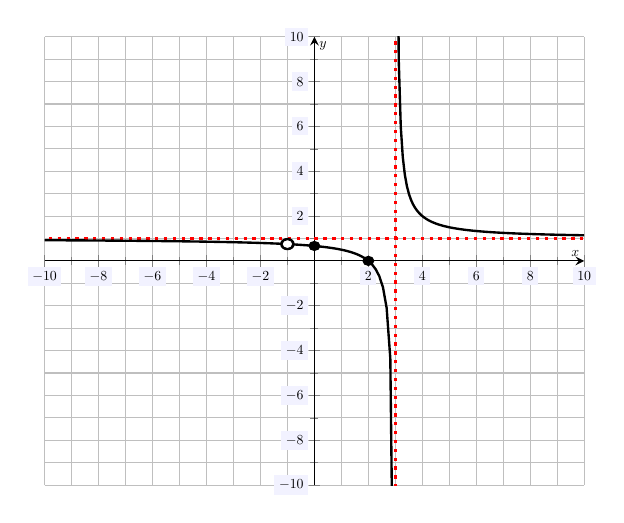
\begin{tikzpicture}[scale=1,every node/.style={scale=0.5}]
	\begin{axis}[
	grid=both,
	axis lines=middle,
	ticklabel style={fill=blue!5!white},
	xmin= -10, xmax=10,
	ymin= -10, ymax=10,
	xtick={-10,-8,...,10},
	ytick={-10,-8,...,10},
	minor x tick num = 1,
	minor y tick num = 1,
	xlabel=\(x\),ylabel=\(y\),
	]
	\draw[fill=black] (0,2/3) circle (0.2);	% y-int
	\draw[fill=black] (2,0) circle (0.2);	% x-int

	\draw[dotted,red, very thick] (3,-10.5) -- (3,10.5);	% Vert Asym
	\draw[dotted,red, very thick] (-10.5,1) -- (10.5,1);	% Horz Asym
	
	% Function
	\addplot[domain= -10.5:2.95,samples=100,line width=0.03cm] ({x}, {(x - 2)/(x - 3)});
	\addplot[domain= 3.05:10.5,samples=100,line width=0.03cm] ({x}, {(x - 2)/(x - 3)});
	
	% After function for overlap
	\draw[fill=black] (-1,3/4) circle (0.25);	% hole
	\draw[fill=white] (-1,3/4) circle (0.2);	% hole
	\end{axis}
	\end{tikzpicture}
	}
	\]

{\itshape\small How do we sketch a rational function? Well, we know how to find `all' the interesting things about it: domain, zeros, asymptotes, holes, etc. So, we can find all these and use this to `fill in' the plot! First, observe\dots
	\[
	\dfrac{x^2 - x - 2}{x^2 - 2x - 3}= \boxed{\dfrac{(x - 2)(x + 1)}{(x - 3)(x + 1)}} \quad '= \, ' \; \dfrac{(x - 2)\cancel{(x + 1)}}{(x - 3)\cancel{(x + 1)}}= \boxed{\dfrac{x - 2}{x - 3}}
	\]
Domain: The domain is where the original denominator is not 0. Solving $(x - 3)(x + 1)= 0$, we see $x= -1, 3$. Therefore, the domain is $\mathbb{R} \setminus \{ -1, 3 \}$. \par\vspace{0.3cm}

$y$-intercept: The $y$-intercept will be the value when $x= 0$. But we have $f(0)= \tfrac{0 - 0 - 2}{0 - 0 - 3}= \tfrac{-2}{-3}= \tfrac{2}{3}$. Therefore, the $y$-intercept is $y= \tfrac{2}{3}$, so we should be sure to include $(0, \tfrac{2}{3})$ on our graph! \par\vspace{0.3cm}

$x$-Intercepts: The $x$-intercepts are the solutions to $f(x)= 0$. For a rational function, this will be when the numerator is 0. Setting $(x - 2)(x + 1)= 0$, we have $x= -1, 2$. But $x= -1$ is not in the domain, and so it cannot be a 0. Therefore, the only $x$-intercepts is $x= 2$. So, we should include the point $(2, 0)$ on our graph. \par\vspace{0.3cm}

Vertical Asymptotes: The vertical asymptotes will occur when the denominator is 0 in the `reduced' rational function. So, we solve $x - 3= 0$, which implies $x= 3$. Therefore, we should sketch a vertical asymptote at $x= 3$. We can even determine how the function approaches this vertical asymptote on the left/right by creating a `sign chart' of the original rational function. We have\dots
	\[
	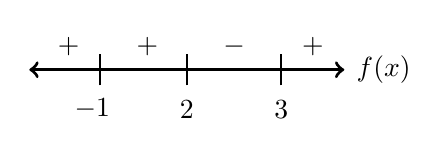
\begin{tikzpicture}
	% Line & Label
	\node at (2.5,0) {$f(x)$};
	\draw[very thick,<->] (-2,0) -- (2,0);
	% -1 label
	\node at (-1.2,-0.5) {$-1$};
	\draw[thick] (-1.1,-0.2) -- (-1.1,0.2);
	% 2 label
	\node at (0,-0.5) {$2$};
	\draw[thick] (0,-0.2) -- (0,0.2);
	% 3 label
	\node at (1.2,-0.5) {$3$};
	\draw[thick] (1.2,-0.2) -- (1.2,0.2);
	% Signs
	\node at (-1.5,0.3) {$+$};
	\node at (-0.5,0.3) {$+$};
	\node at (0.6,0.3) {$-$};
	\node at (1.6,0.3) {$+$};
	\end{tikzpicture}
	\]
So, the graph should `go down to $-\infty$' as it approaches the vertical asymptote on the left, and `go up to $+\infty$' as it approaches the vertical asymptote on the right. 

Horizontal Asymptote: Examining the original rational function, the numerator has degree 2 and the denominator has degree 2. Therefore, the horizontal asymptote will be the ratio of the leading coefficients, which is $\tfrac{1}{1}= 1$. Therefore, $y= 1$ is the only horizontal asymptote. We should draw this horizontal asymptote and be sure the function approaches this asymptote as it moves `further to the left and right.' \par\vspace{0.3cm}

Holes: To find holes, we examine values not in the domain where the denominator is not 0 in the `reduced' rational function. The only such value here is $x= -1$. Therefore, the only hole is at $x= -1$. The $y$-value will be the $y$-value at this $x$-value in the `reduced' rational function. This is $\tfrac{-1 - 2}{-1 - 3}= \tfrac{-3}{-4}= \tfrac{3}{4}$. Therefore, the hole is $(-1, \tfrac{3}{4})$, which we should include in our graph. \par\vspace{0.3cm}

Putting all these features together gives us the plot above.
}

\end{document}